\documentclass[utf8,1pt]{extarticle} % Use extarticle for more font size options 

\usepackage[utf8]{inputenc}
\usepackage{graphicx} % Required for including images
\usepackage{amsmath, amssymb} % Required for math features
\usepackage{hyperref} % For hyperlinks
\usepackage{natbib} % For bibliography
\usepackage{geometry} % For page dimensions and margins
\geometry{a4paper, margin=1.2in}

\title{Machine Learning Project Report: Neural Network Implementation on MNIST Dataset}
\author{Noé Bourgeois}
\date{Academic Year 2023-2024}

\begin{document}

\maketitle

\newpage
\section{Introduction}
This report details a neural network's development and analysis for digit recognition using the MNIST dataset, highlighting key findings and future research directions.
\section{Experimentation Framework}
For the framework base,
please see the instructions.
\subsection{Batching}
We used batching from 0.5 to 1e-5
to reduce the training process memory need and increase noisy data able accuracy.
 
 \subsection{Learning rate}
 Reducing the batch size requires to lower the learning rate proportionally.
 The learning rate can also be augmented with the neurons quantity or the loss
 and reduced with the epochs or the fitness

 \subsection{Weights}
\subsubsection{Weight Restoration}
The network can memorize the training lowest loss weights and revert to the memorized weights. 

\section{Results}
\subsection{Training}
% \begin{figure}
%     \centering
%     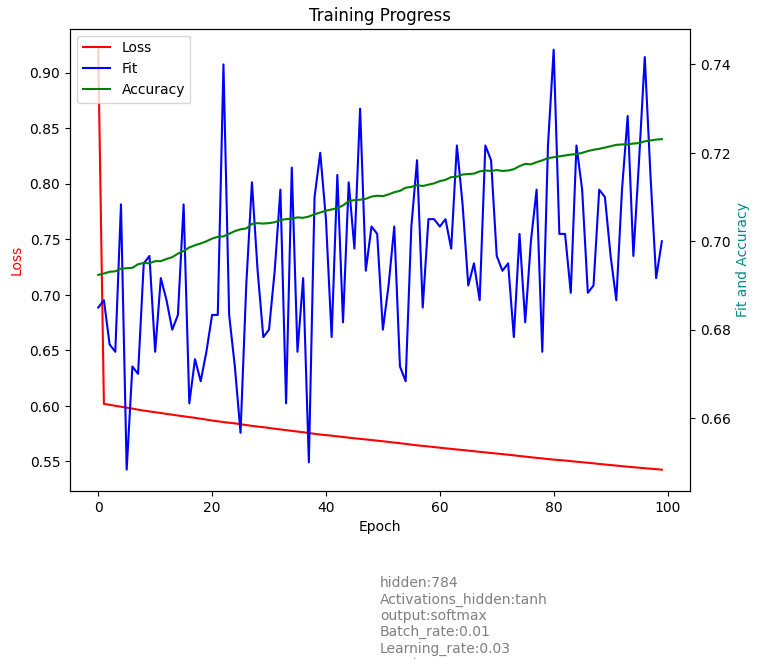
\includegraphics[width=0.8\textwidth]{media/training/progress/_hidden_784_Activations_hidden_tanh_output_softmax_Batch_rate_0.01_Learning_rate_0.03_Epochs_100_Loss_0.5568668422941822_Fit_0.7.png}
%     \label{fig:comparison}
%     \
% \end{figure}
\begin{figure}
    \centering
    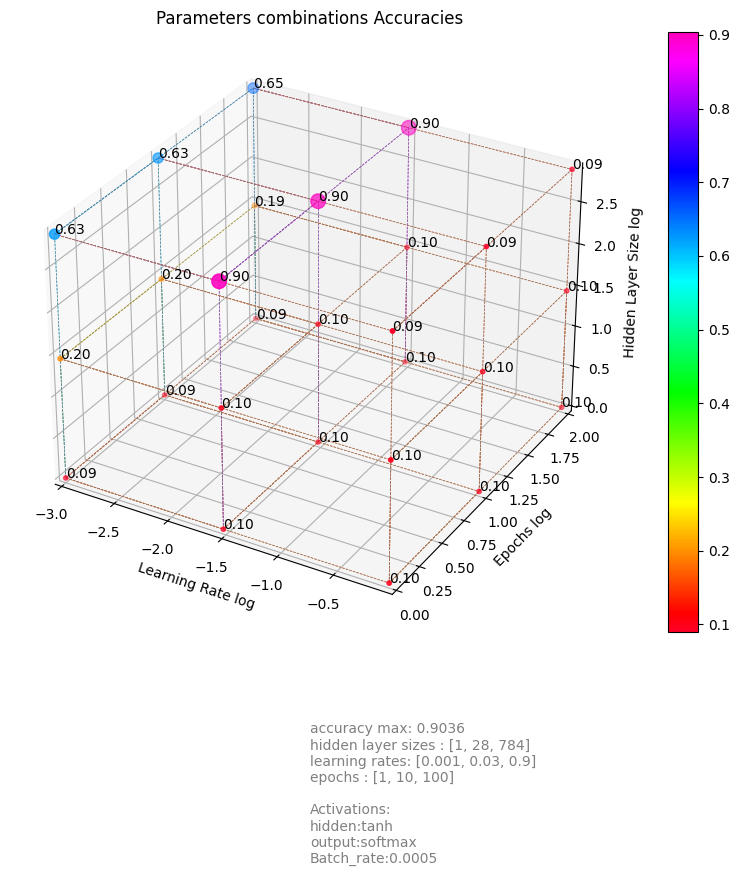
\includegraphics[width=0.8\textwidth]{media/training/accuracy_max_0.90_min_0.09__Activations__hidden_tanh_output_softmax_Batch_rate_0.0005_Epochs_89.png}
    \label{fig:comparison}
\end{figure}
\subsection{Testing}
\subsubsection{Confusion Matrix}
% graph:
\begin{figure}
    \centering
    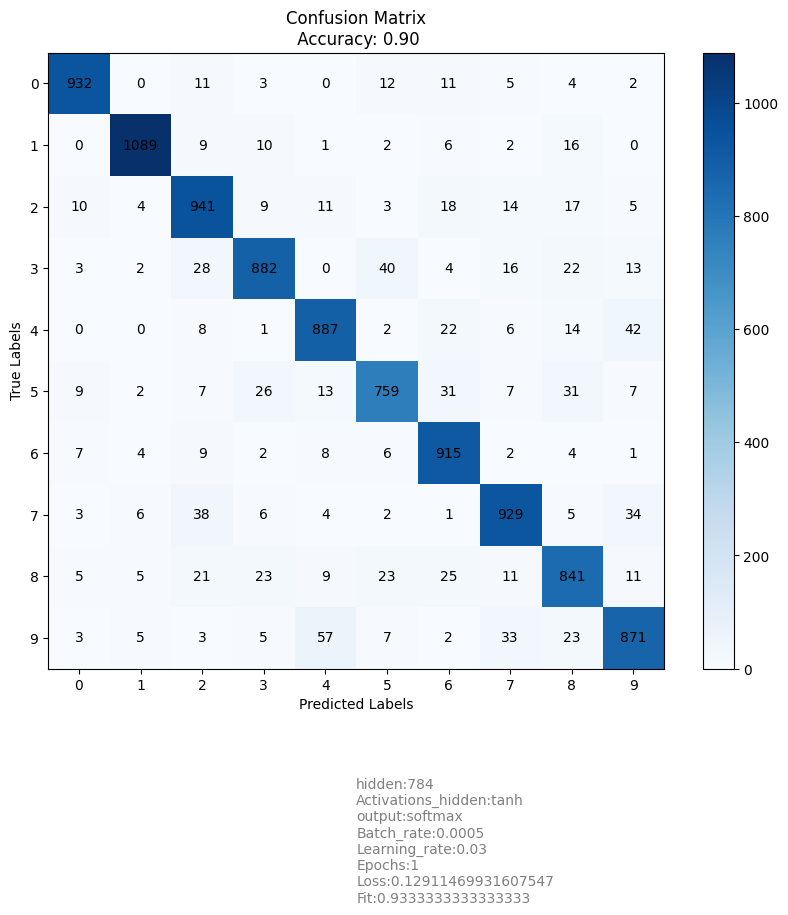
\includegraphics[width=0.8\textwidth]{media/confusion/_hidden_784_Activations_hidden_tanh_output_softmax_Batch_rate_0.0005_Learning_rate_0.03_Epochs_1_Loss_0.12911469931607547_Fit_0.9333333333333333.png}
    \label{fig:confusion}
\end{figure}
\subsection{Convolution}
With a convolutional model, we achieved
98.8\% accuracy
in 1 minute and 40 seconds.
to compare, the best accuracy we achieved with a non-convolutional model was 91\% in 1 minute and 40 seconds.

\section{Analysis}
The "parameters combinations accuracies" results plots indicate a strong dependency of our
neural network performance on its 
size, we can clearly see that color shadind on the vertical axis.
The learning rate, whose calculation was optimized for 784 neurons and becomes even more fragile with batch size reduction also has a strong impact on the accuracy.
Even at this same size, a milli scale variation separates near- maximum and maximum accuracy.
During training, micro scale variations determines the accuracy evolution. 
The epochs quantity allows the accuracy to evolve, but only positively if the learning rate is adapted.
Otherwise, stagnation or overfitting occurs.

\section{Conclusion}
\subsection{Main Findings}
To be concise, 
the biggest challenge being to constantly adpapt the learning rate,
we conclude that a biggest network allowing high and fast performance (to 90\% accuracy after 1 epoch),
smallest batching catalyzing that behavior on noise and
a learning rate adapted to network and batch size, and dynamically to loss.
should be preffered.
That having been said, many other techiques can be added to improve the model's time complexity. 
\subsection{Tools}
\begin{itemize}
    \item ChatGPT
\end{itemize}
\subsection{Future Work}
We will continue Implementing advanced techniques like filtering images on sparse matrices,
biases, batch normalization- and dropout regularization- at different intensities
at particular network states and exploring convolutional models and
deeper pattern finding architectures.

The project is available on \href{https://github.com/nobourge/artificial-intelligence-machine-learning}{https://github.com/nobourge/artificial-intelligence-machine-learning}.


% \section{References}
% % Include your references here
% %links:

% https://medium.com/france-school-of-ai/math%C3%A9matiques-des-r%C3%A9seaux-de-neurones-code-python-613d8e83541
% https://lrpserver.hhi.fraunhofer.de/handwriting-classification

% \bibliographystyle{plain}
% \bibliography{references} % references.bib should be the name of your BibTeX file

\end{document}
